\documentclass[../mech.tex]{subfiles}
\graphicspath{{\subfix{../figures/}}}
\begin{document}
\chapter{Kinematics}
\section{Scalars and Vectors}
Scalars are quantities described by magnitude only, vectors are quantities described by both magnitude and direction.

Vectors can be visually modeled as arrows with appropriate direction and lengths proportional to their magnitudes.

Vectors can be expressed in unit vector notation or as a magnitude and a direction.
\begin{itemize}
    \item Unit vector notation can be used to represent vectors as the sum of their constituent components in the x, y, and z directions, denoted by $\hat{i}, \hat{j}$ and $\hat{k}$.
    \[ \vec{r} = A\hat{i}+B\hat{j}+C\hat{k}\]
    \item The position vector of a point is given by $\vec{r}$ and the unit vector in the direction of the position vector is denoted $\hat{r}$.
    \item A resultant vector is the vector sum of the addend vectors' components. 
    \[ \vec{C}=\vec{A}+\vec{B}=(A_x+B_y)\hat{i}+(A_y+B_y)\hat{j} \]
\end{itemize}

In a given one-dimensional coordinate system, opposite directions are denoted by opposite signs.

\begin{example}
    If $\vec{a}=3\hat{i}+4\hat{j}-\hat{k}$ and $\vec{b}=-2\hat{i}+\hat{y}+2\hat{k}$, what is 
    (a) $\vec{c}=\vec{a}+\vec{b}$

    $\vec{c}=(3+-2)\hat{i}+(4+1)\hat{j}+(-1+2)\hat{k}=\hat{i}+5\hat{j}+\hat{k}$

    (b) $\vec{c}=\vec{a}-\vec{b}$

    $\vec{c}=(3+2)\hat{i}+(4-1)\hat{j}+(-1-2)\hat{k}=5\hat{i}+3\hat{j}-3\hat{k}$

    (c) $\vec{c}=\vec{b}-\vec{a}$

    $\vec{c}=(-2-3)\hat{i}+(1-4)\hat{j}+(2+1)\hat{k}=-5\hat{i}-3\hat{j}+3\hat{k}$
\end{example}

\ex An object moves in the $xy$-plane a distance $A$ at an angle $\theta$ measured counterclockwise from the positive $x$-direction, where $0<\theta<90\degree$. The object then moves a 
distance $B$ in the positive $x$-direction. The change in the $x$-component of the object's position is equal to the change in the $y$-component of its positions. What is $B$ in terms of $A$ and $\theta$?

\ex An object is moving with an initial velocity $\vec{v}_1=(3.00\hat{i}+4.00\hat{j})$ m/s. After a certain time interval, its velocity is $\vec{v}_2=(-8.00\hat{i}+15.0\hat{j})$ m/s. What is the magnitude of the change in the velocity of the object over this time interval?

\section{Displacement, Velocity, and Acceleration}
When using the object model, the size, shape and internal configuration are ignored.
\begin{itemize}
    \item The object may be treated as a single point with extensive properties such as mass and charge.
\end{itemize}
Displacement is the change in an object's position: $\Delta x = x-x_0$

Averages of velocity and acceleration are calculated considering the initial and final states of an object over an interval of time.

Average velocity is the displacement of an object divided by the interval of time in which that displacement occurs:
\[ \vec{v}_{avg}=\frac{\Delta \vec{x}}{\Delta t}\]
Average acceleration is the change in velocity divided by the interval of time in which that change in velocity occurs.
\[ \vec{a}_{avg}=\frac{\Delta \vec{v}}{\Delta t}\]
As the time interval used to calculate the average value of a quantity approaches zero, the average value of that quantity approaches the value of the quantity that is instant, called the instantaneous value.
\begin{itemize}
    \item $\vec{v} = \frac{\dd x}{\dd t}$
    \item $\vec{a} = \frac{\dd v}{\dd t}$
\end{itemize}

Time dependent functions and instantaneous values of position, velocity and acceleration can be determined using differentiation and integration.

\begin{example}
    A particle moves along the $x$-axis with an acceleration of $a=18t$, where $a$ has units of m/s$^2$. If the particle at $t=0$ is at the origin with a velocity of $-12$ m/s, what is its position at $t=4.0$ s?

    The velocity is the integral of acceleration: $v=\int 18t \dd t = 9t^2+C$. Substituting the initial conditions gives $v(0)=-12$.

    Integrating the velocity function: $\int 9t^2-12\dd t = 3t^3-12t+C$.

    Since we know $x(0)=0$, plug this in and we find that $C=0$. Therefore, $x(4)=144$ m.
\end{example}

\ex An object moves in one dimension along the $x$-axis. At time $t=0$, the object is located at position $x=1$ m and has a velocity of $v=1$ m/s. The object's acceleration varies 
as $a=3t$, where $a$ is in m/s$^2$ and $t$ is time in seconds. A student incorrectly derives the equation for the object's position as $x=\frac{1}{2}t^3+1$ where $x$ is in meters. What is a possible error that could have resulted in the incorrect equation?

\ex Two objects, Object 1 and Object 2, have velocities $\vec{v}_1=(3t^2\hat{i}+5t\hat{j})$ m/s and $\vec{v}_2=(5t^2\hat{i}-3t\hat{j})$ m/s, respectively, where $t$ is time in seconds. What is the relationship between the magnitudes of the acceleration $a_1$ 
of Object 1 at $t=1$ s and the acceleration $a_2$ of Object 2 at $t=1$ s?

\section{Representing Motion}
Motion can be represented by motion diagrams, figures, graphs, equations and narrative descriptions.

For constant acceleration, three kinematics equations can used to describe the instantaneous linear motion in one dimension:
\begin{itemize}
    \item $v=v_0 + at$
    \item $x=x_0+v_0 t + \frac{1}{2}at^2$
    \item $v^2=v_0^2+2a\Delta x$
\end{itemize}

Near the surface of the Earth, the vertical acceleration caused by the force of gravity is downward, constant and has a measured value of $g=9.8$ m/s$^2$ or $g=10$ m/s$^2$.

Graphs of position, velocity and acceleration as functions of time can be used to find the relationships between those quantities.
\pagebreak
\begin{example}
    A large cat, running at a constant velocity of 5.0 m/s in the positive $x$ direction, runs past a small dog that is initially at rest. Just as the cat passes the dog, the dog begins accelerating at 0.5 m/s$^2$ in the positive $x$ direction.
    (a) How much time passes before the dog catches up to the cat?

    We know from the formula $x=v_0t+\frac{1}{2}at^2$ that the cat will have position $5t$ and the dog $0.25t^2$.

    Setting these equal to each other gives $t=20$ s.

    (b) How far has the dog traveled at this point?

    Plug in $t=20$ s to get $100$ m.

    (c) How fast is the dog traveling at this point?

    The formula $v=v_0+at$ can be used to get $10$ m/s.
\end{example}

\ex \begin{center}
    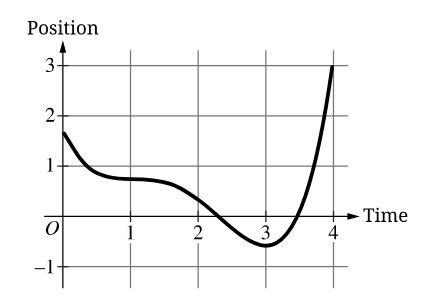
\includegraphics[width=0.5\textwidth]{1.3.PNG}
\end{center}
An object moves in one dimension along the $x$-axis as described by the position versus time graph shown in the figure. During the time interval of the graph, how many times does the object change direction and what feature or features of the graph justifies this response?

\ex On a distant planet where the acceleration due to gravity is $g_P$, an object takes a time $t_P$ to reach the ground when dropped from a height $h_0$. On a small moon of the planet, the acceleration due to gravity is $\frac{g_P}{16}$. How long does it take an object to reach the ground when it is dropped from the same height on the moon?

\section{Reference Frames and Relative Motion}
The choice of reference frame will determine the direction and magnitude of quantities measured by an observer in that reference frame.

Measurements from a given reference frame may be converted to measurements from another reference frame.

The observed velocity of an object results from the combination of the object's velocity and the velocity of the observer's reference frame.
\begin{itemize}
    \item Combining the motion of an object and the motion of an observer in a given reference frame involves the addition or subtraction of vectors.
    \item The acceleration of any object is the same as measured from all inertial reference frames.
\end{itemize}

\pagebreak
\begin{example}
    A cat passes a dog, traveling in the positive $x$-direction at 5.0 m/s. As the cat passes, the dog begins accelerating at 0.5 m/s$^2$ in the positive $y$-direction.

    (a) What is the cat's acceleration relative to the dog?

    The acceleration of the cat relative to the ground is $0\hat{i}$ and the acceleration of the dog relative to the ground is $0.5\hat{j}$ so the acceleration of the cat relative to the dog is $0\hat{i}-0.5\hat{j}$.
    
    (b) What is the cat's velocity relative to the dog at time $t=5.0$ seconds after the dog begins running?

    We have $v=v_{cat}+a_{CD}t = (5\hat{i}-2.5\hat{j})$ m/s 

    (c) What is the cat's position relative to the dog at $t=5.0$ seconds after the dog begins running?
    
    From $\Delta r = v_{CD}t+\frac{1}{2}a_{CD}t^2$, we get that $\Delta r = 25\hat{i}-6.25\hat{j}$.
\end{example}

\ex A toy plane which maintains an airspeed $v_p$ flies between points $A$ and $B$ in a time $t_0$ when there is negligible wind. When the air is moving at a velocity of $\frac{1}{2}v_p$ from 
point $B$ to point $A$, the toy plane can make the trip from $A$ to $B$ in $t_{AB}$, and the return trip from $B$ to $A$ in $t_{BA}$. How do the three travel times compare?

\ex Car $A$ is traveling east with a speed of 30 m/s. Car B is traveling north with speed of 40 m/s. What is the direction of the velocity of Car B relative to Car A?

\section{Motion in Two or Three Dimensions}
Motion in two or three dimensions can be analyzed using one-dimensional kinematic relationships if the motion is separated into componenets.

Velocity and acceleration may be different in each dimension and be nonuniform.

Motion in one dimension may be changed without causing a change in the perpendicular dimension.

Projectile motion is a special case of two-dimensional motion that has zero acceleration in one dimension and constant, nonzero acceleration in the second dimension.

\begin{example}
    The motion of an object can be described by the equations 
    \begin{itemize}
        \item $x(t)=4t^2-3t$
        \item $y(t)=3t^3-2t^2-9t$
    \end{itemize}

    (a) What is the objects displacement after 2.5 s?

    Plug in $t=2.5$ for both equations to get $\Delta \vec{r}=(17.5\hat{i}+11.9\hat{j})$ m.

    (b) Find the two equations that describe the object's velocity in the $x$ and $y$ directions.

    Take the derivative of both equations to get $v_x=8t-3$ and $v_y=9t^2-4t-9$.

    (c) What is the object's velocity after 2.5 s?

    Plug in 2.5 to both equations from part (b) to get $v=(17\hat{i}+37.25\hat{j})$ m/s.
\end{example}

\ex Object 1 is launched at an initial speed $v_0$ at an angle $\theta$ above the horizontal and reaches a maximum height of $y_1$. Object 2 is launched at an initial speed $2v_0$ at the same angle $\theta$, reaching a maximum height of $y_2$. What is the relationship between $y_1$ and $y_2$?

\pagebreak
\ex \begin{center}
    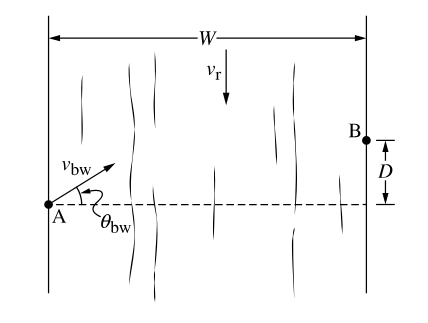
\includegraphics[width=0.5\textwidth]{1.5.PNG}
\end{center}
A river has width $W$ and a current $v_r$. A boat maintains a constant velocity as it travels from Point A to Point B. Point B is located at a distance $D$ upstream from point A. The boat's water speed is 
$v_{bw}$ with a heading of angle $\theta_{bw}$, as shown in the figure. What is a correct expression for $D$?

\end{document}